\chapter{The transcriptional Landscape of \cer{}}
The rise of microarrays and next generation sequencing techniques has made the exploration of the transcriptome possible. 
Early application of tiling arrays to the transcriptome of S.cerevisiae showed that, in addition to protein coding genes and a multitude of functional non-coding RNAs, the genome is pervasively transcribed and RNA molecules can arise from many unannotated regions \cite{xu:2009:bidirectional, neil:2009:widespread,david:2006:highresolution}. 
There are multiple possible reasons for this phenomenon. 
The genome might provide an inherently low barrier to transcription initiation. 
Additionally, studies have shown that yeast promoters, despite showing directionality, can fire bidirectionally and give rise to non-functional RNAs \cite{xu:2009:bidirectional, neil:2009:widespread}. 
Promoter bidirectionality, and the general propensity of transcription to initiate spuriously, is at the origins of the widespread occurrence of transcription, which is usually referred to as pervasive transcription and contributes to the generation of large quantities of non-coding (mostly non-functional) RNAs. 

\section{Control of pervasive transcription}

Pervasive transcription represents a non-negligible fraction of all RNAPII transcription. 
Therefore, it has the potential to interfere with other physiological events and needs to be carefully regulated. 
Control of pervasive transcription occurs on two levels: First, RNAPII that initiates spuriously need to be rapidly terminated, in order to avoid interference with other processes on DNA; second, the resulting transcripts need to be efficiently degraded, to prevent accumulation of toxic species. 

The NNS complex is the main termination pathway involved in control of pervasive transcription \cite{arigo:2006:regulation, thiebaut:2006:transcription}. 
Binding sites for Nrd1 and Nab3 are frequently enriched in areas where pervasive transcription occurs, such as antisense to coding RNAs and in intergenic regions \cite{thiebaut:2006:transcription}. 
Acting early in the transcription cycle, NNS is an effective tool to block such transcription events before they can do damage. 
Despite the major role of NNS, CPF-CF, as well as some non-canonical termination pathways, have been implicated in termination of pervasive transcription \cite{marquardt:2011:distinct, vandijk:2011:xuts,colin:2014:roadblock}.

Once termination has occurred, transcripts are released into the nucleus. 
These RNA species do not possess coding potential and might be deleterious to the cell if accumulated in sufficient quantities. 
In order to prevent such accumulation, the cell evolved RNA quality control systems that can degrade spurious and aberrant transcripts. 
These decay pathways can be directly connected to termination and 3’ processing, as in the case of NNS and the TRAMP-Exosome \cite{thiebaut:2006:transcription}, or recognize specific features that mark non-functional transcripts, such as poor coding potential.

\section{Classes of pervasive transcript} \label{pervasiveTranscripts}

Because of their rapid turnover, the majority of pervasive transcripts are difficult to detect in wild type cells. 
Several studies found that deletion of certain elements of RNA quality control would affect the stability of only a subset of pervasive transcripts, making them appear in transcriptome analyses \cite{wyers:2005:cryptic, vandijk:2011:xuts}. 
Over time, it became obvious that several classes exist, each responding differently to inactivation of specific quality control pathways. 
The following classes, therefore, represent sets of transcripts sharing one or more features that make them more susceptible to specific branches of quality control.

\begin{figure}[ht]

\centering
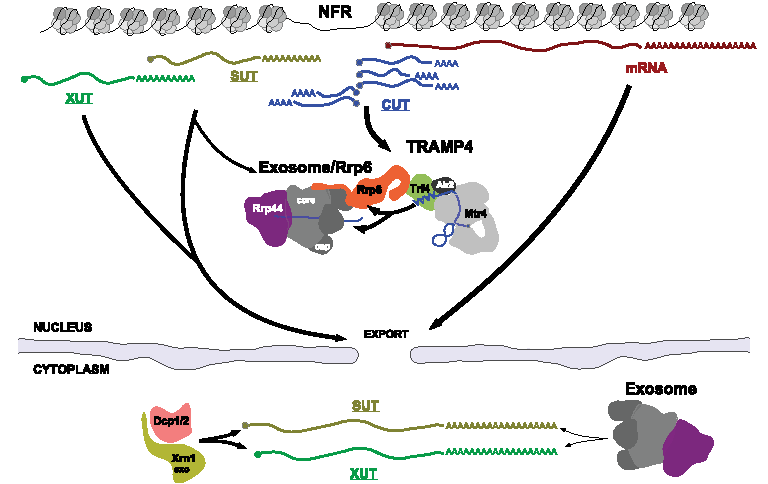
\includegraphics[width=\textwidth]{figures/introduction/pervasiveTr}
\caption[Classes of transcripts and their fates.]{The cellular fate of pervasive transcripts. Different classes of non-coding RNAs are represented at the top. Black arrows indicate the fate of the transcript after transcription, either immediate degradation via the exosome/\gls{tramp} quality control pathway, or export to the cytoplasm. Here, cytoplasmic quality control is shown.}
\label{fig:pervasiveTranscripts}

\end{figure}


\paragraph{CUTs}

The first—and most abundant—class of pervasive transcripts to be described, Cryptic Unstable Transcripts (CUTs) were identified in a strain missing the exosome co-factor Rrp6 \cite{wyers:2005:cryptic}. 
CUTs are short transcripts (400-800 bp) originating from intergenic regions and bidirectional promoters.
They can often be detected in the antisense direction to protein coding genes and their transcription can sometimes contribute to gene regulation \cite{arigo:2006:termination}. 

CUTs are terminated by the NNS pathway \cite{arigo:2006:regulation}. 
This greatly facilitates their turnover, which occurs exclusively in the nucleus. 
After transcription termination has occurred, CUTs are contacted by TRAMP and handed over to the nuclear exosome, resulting in their rapid degradation \cite{thiebaut:2006:transcription}.

\paragraph{SUTs}

Unlike CUTs, Stable Untranslated Transcripts (SUTs) are detectable in wild type cells \cite{david:2006:highresolution}. 
This difference is due to the termination mechanism that characterizes these transcripts. While CUTs are terminated early by the NNS pathway, SUTs are longer and terminate through the CPF-CF pathway \cite{marquardt:2011:distinct}. 
This difference in termination implies that SUTs can more easily escape the nucleus and be exported into the cytoplasm. 
It should be noted that a large portion of SUTs is partially affected by exosome mutations, suggesting that multiple termination mechanisms might contribute to the generation of these transcripts. 

Despite being exported to the cytoplasm, SUTs have poor coding potential and are targeted by specific quality control pathways in this compartment (see below) \cite{malabat:2015:quality}.

\paragraph{XUTs}

Very close to SUTs, Xrn1-dependent Unstable Transcripts (XUTs) have essentially the same characteristics.
They are terminated by the CPF-CF pathway and rapidly exported to the cytoplasm \cite{vandijk:2011:xuts}. 
However, while the turnover rate of SUTs is sufficiently slow to allow their detection in wild type cells, XUTs are more susceptible to cytoplasmic decay pathways, and therefore require deletion of Xrn1—the main molecular effector of cytoplasmic RNA degradation—to become visible in transcriptome analyses \cite{vandijk:2011:xuts},=.


\paragraph{NUTs}

Largely overlapping with CUTs, Nrd1-dependent Unterminated Transcripts (NUTs) are defined as transcripts that gain stability when NNS termination is impaired \cite{schulz:2013:transcriptome}. 
Normally, these transcripts are rapidly degraded by the nuclear exosome. 
However, when NNS termination is impaired, they gain in length and stability, becoming detectable.

\paragraph{RUTs}

Only recently identified as a new class of pervasive transcripts, Reb1-dependent Unstable Transcripts (RUTs) are transcripts subjected to road-block termination by the transcription factor Reb1 and subsequently degraded by the nuclear exosome \cite{colin:2014:roadblock}.

\section{Quality control pathways}

RNA quality control eliminates aberrant and pervasive transcripts through degradation. 
Several multisubunit complexes located throughout the cell carry out this function through use of endo- and exo-nuclease activities. 
Targeting of transcripts to these complexes (i.e. marking for degradation) can occur through several means: it can be directly connected to the termination mechanism used to release the transcript (as in the case of NNS termination), or it can depend on certain features of the RNA, such as presence of a premature stop codon.

The exosome is known to act in both the nucleus and the cytoplasm. 
Its catalytic activity depends on the subunit Dis3, which possesses 3' to 5' exonuclease and endonuclease activity. In the nucleus, the exosome is associated with two specific co-factors: a second 3' to 5' exonuclease called Rrp6, and a polyadenylation complex called TRAMP \cite{lacava:2005:rna}. 
While Rrp6 significantly contributes to RNA degradation through its exonuclease activity, TRAMP stimulates the activity of the exosome through addition of short poly(A) tails and other, less clear means \cite{haracska:2005:trf4,jia:2012:rna}. 
This ensemble of factors makes the exosome the foremost quality control agent in the nucleus. 
In the cytoplasm, the exosome is not found in complex with Rrp6 or TRAMP and has only a minor role in RNA degradation \cite[for review see][]{tudek:2015:noncoding}.

In the cytoplasm, RNA degradation is mainly enforced by the 5' to 3' exonuclease Xrn1. 
Several decay pathways can lead to degradation by Xrn1 (and to some extent the cytoplasmic exosome): Non-sense Mediated mRNA Decay (NMD), triggered by the presence of a premature stop codon; No-Go Decay (NGD), triggered by lack of a translation start codon; and No-Stop Decay (NSD), caused by lack of a stop codon.
These pathways target transcripts that do not possess the typical features of mRNAs, stopping potentially toxic elements from being translated \cite[for review see][]{houseley:2009:many}. 
Xrn1 is known to target pervasive transcripts with poor coding potential, such as SUTs and XUTs, providing a backup system that can deal with those RNAs that manage to escape the nuclear quality control \cite{malabat:2015:quality}.

\section{Function of pervasive transcripts}

The question of whether pervasive transcripts in yeast possess any functional activity remains unclear.
While the act of pervasive transcription has been associated with regulatory events on multiple occasions, very little is known about the function of the transcripts themselves. 

For instance, SER3 expression is known to be regulated by the upstream transcription unit SRG1—producing a non-coding RNA—through a mechanism of transcriptional interference \cite{martens:2004:intergenic}. 
This phenomenon occurs when an elongating polymerase invades a promoter, thereby reducing the efficiency of transcription initation. Similarly, the PHO84 gene seems to be regulated by an antisense transcript that runs along the whole gene, reaching the promoter and downregulating expression \cite{castelnuovo:2013:bimodal}. 
In both these cases, repression is mediated by a modification of the chromatin state of the promoter, which prevents assembly of the Pre-Initiation Complex. Stabilization of the transcript, however, did not in any way affect the repression.

Other regulation mechanisms involve NNS termination and a conditional generation of CUTs. Several nucleotide biosynthesis genes (URA2, URA8, IMD2 among others) can initiate transcription from two regions separated by an NNS terminator sequence \cite{jenks:2008:properties, thiebaut:2008:futile}. 
Only transcription from the downstream TSS results in productive elongation, while transcription starting from the upstream TSS results in early termination and degradation of the transcript. 
It has been shown that nucleotide availability modulates TSS selection, and said genes are properly expressed only when specific nucleotide concentrations are low.


\clearpage



